\documentclass[a5paper]{article}
\usepackage[margin=0pt]{geometry}
\usepackage{fontspec}

\usepackage[dvipsnames]{xcolor}

\definecolor{LCARS0}{HTML}{FFAA00}
\definecolor{LCARS1}{HTML}{577a83}%{7190C6}
\definecolor{LCARS2}{HTML}{B24F46}
\definecolor{LCARS3}{HTML}{41444F}
\definecolor{LCARS4}{HTML}{DE8443}
\definecolor{LCARS5}{HTML}{25272E}

\usepackage{tikz}
\usetikzlibrary{tikzmark}
\usetikzlibrary{calc}

% To create nice looking image, use the high-res background art (retro_endeavour_cover_bg_high_res.png) to make a (big) pdf version of the cover.
% Then export to png and adjust the resolution as needed. For best results, resize to A5 (14.8cm x 21cm) with (at least) 300 dpi resolution.

\begin{document}
	\thispagestyle{plain}
	\begin{center}
	\begin{tikzpicture}[remember picture, overlay]
		\node () at (current page.center) {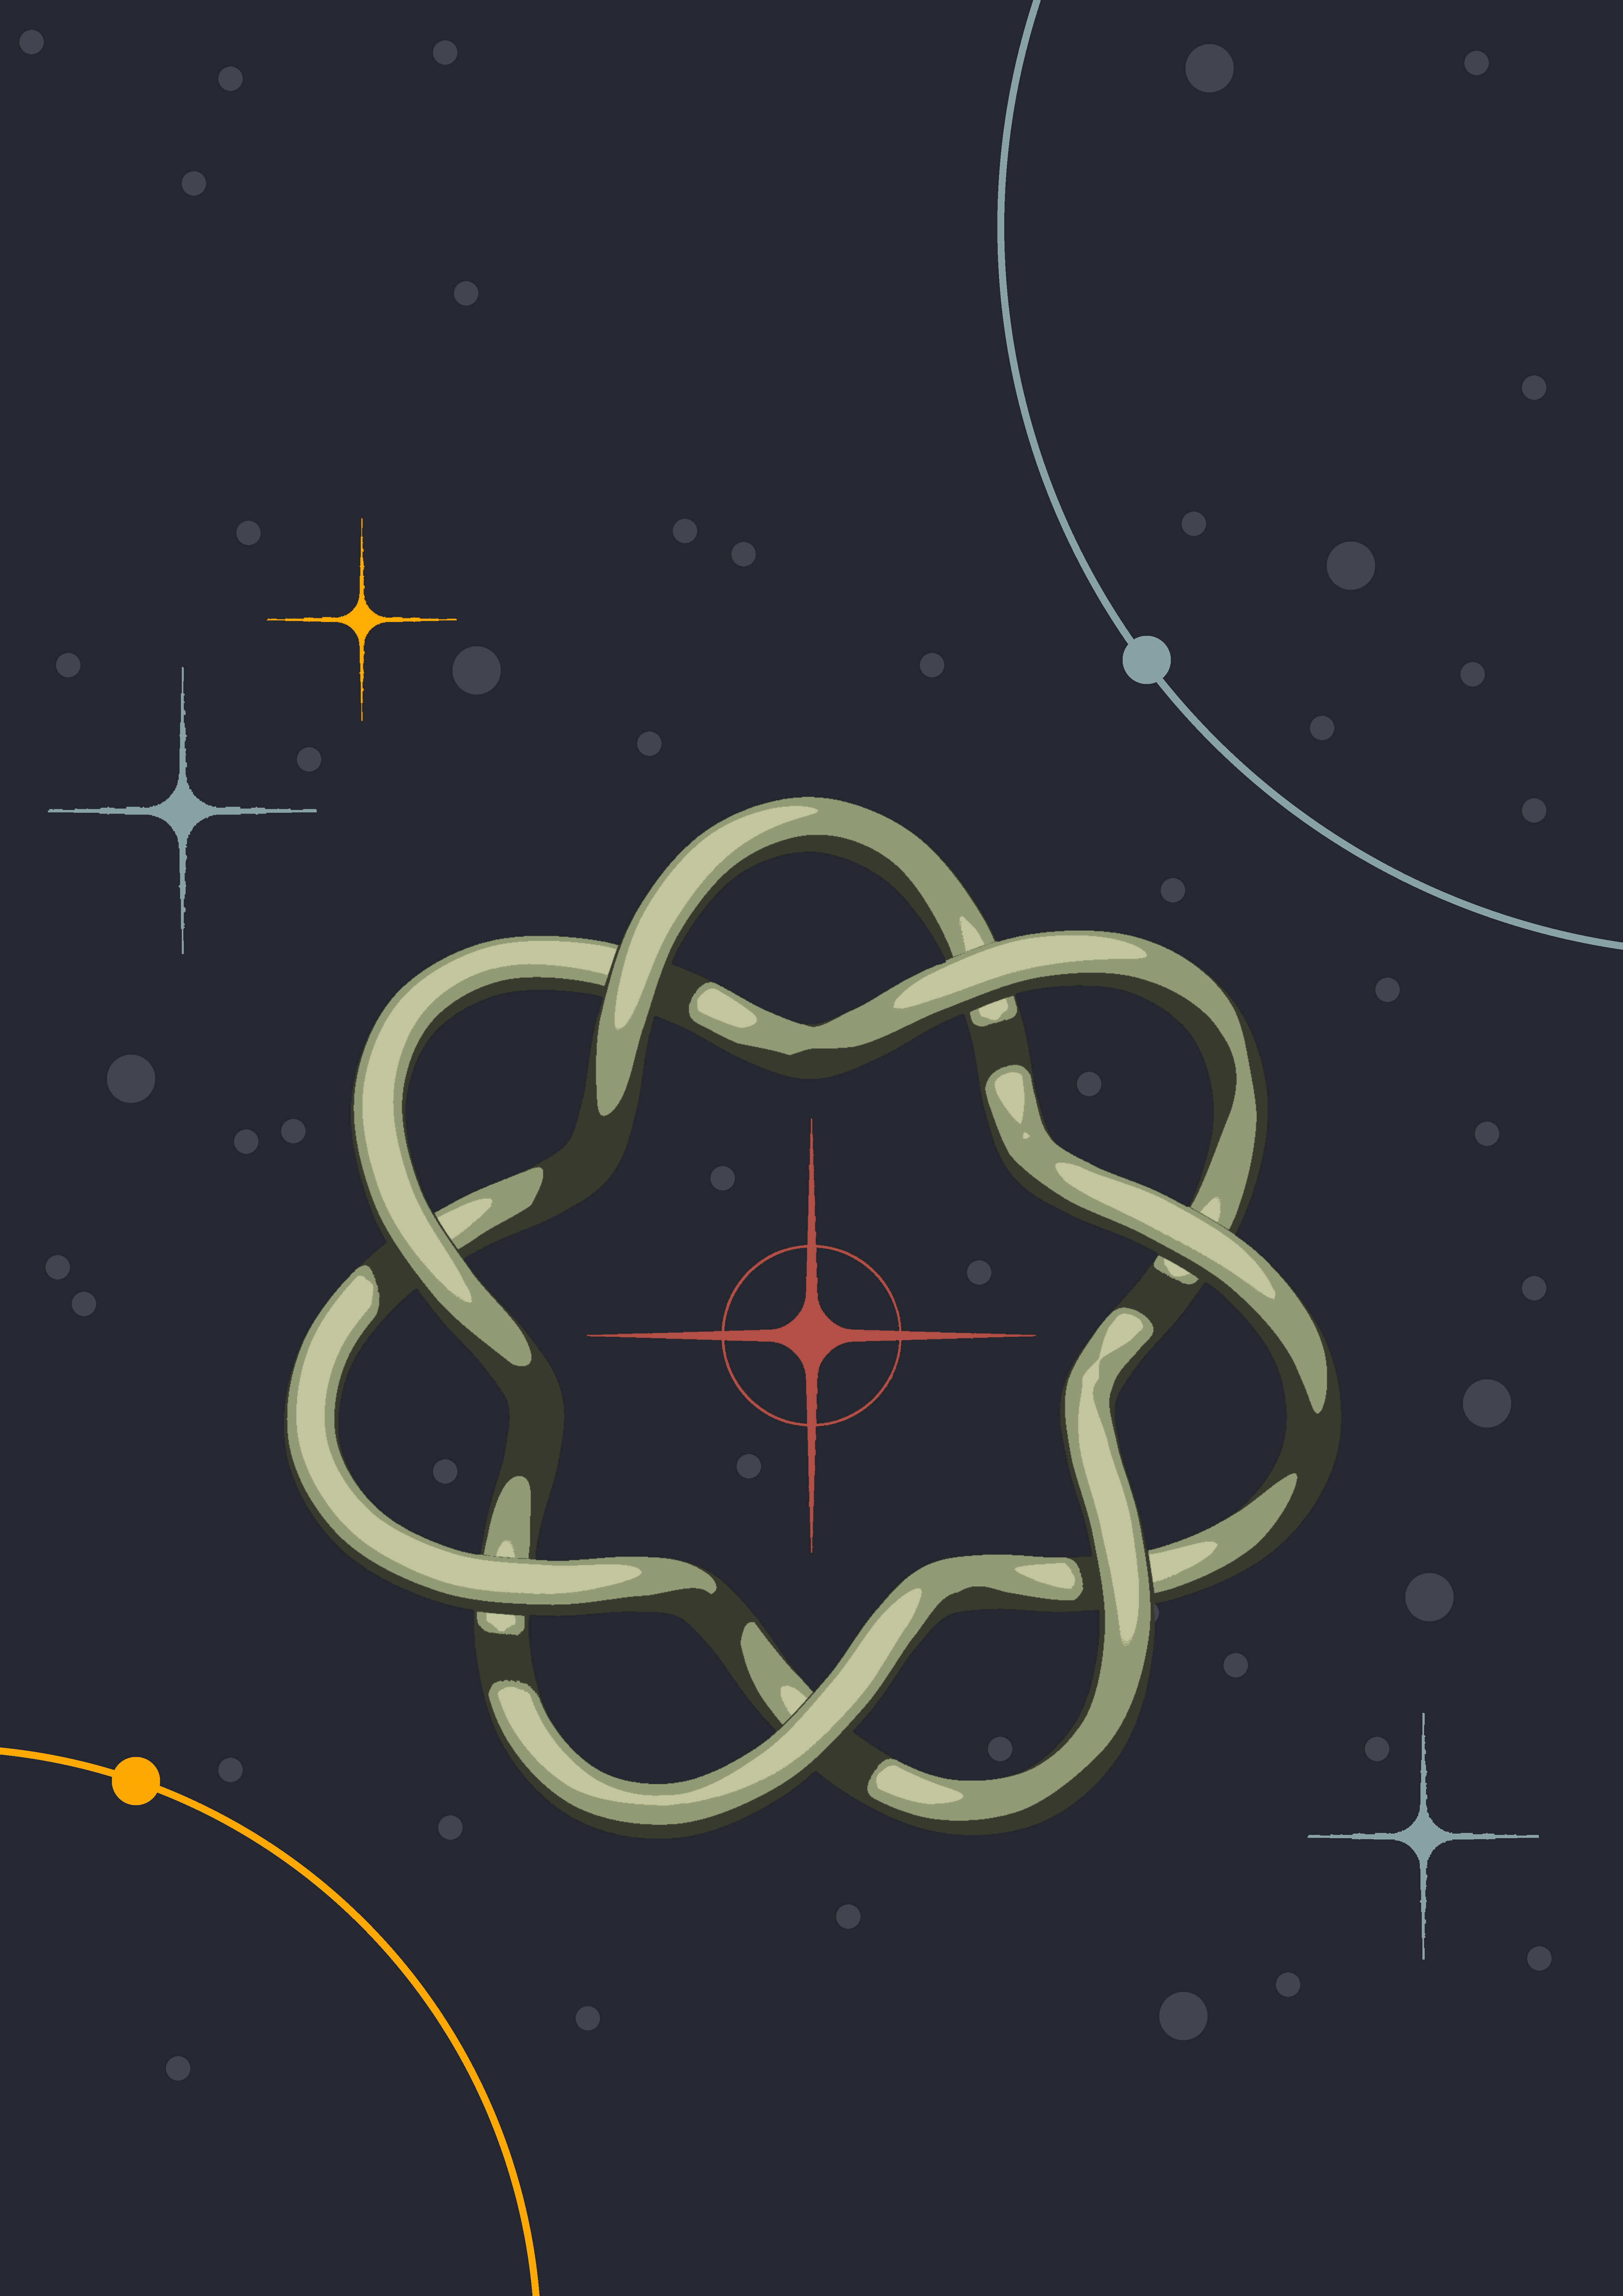
\includegraphics[height=\paperheight, width=\paperwidth]{../Images/torus_knot.png}};

		\setmainfont[Scale=6.5]{TT Mussels-BoldItalic}
		\node[fill=LCARS4, minimum width=\pagewidth, anchor=north] () at (0,-0.8cm) {\textcolor{LCARS5}{{\small OUROBOROUS}}};

		\setmainfont[Scale=2.0]{Futura}
		\node[fill=LCARS5, minimum width=\pagewidth, anchor=south, minimum height=2cm] () at (0,-\pageheight+0.5ex) {\textcolor{LCARS4}{{\small{An ENDEAVOUR Adventure by Paul Murray}}}};
	\end{tikzpicture}
	\end{center}
\end{document}